\section{Introduction}
\label{introduction}

Various types of graphs are commonly used as models for real-world phenomenon, such as online social networks, biological networks, World Wide Web, among others. As their sizes keep increasing, scaling up their algorithms to handle extreme size graphs with billions of vertices and edges remains a challenge that has drawn increased attention in recent years. Specifically, straightforward operations in graph theory are usually too slow or costly when they are applied to graphs at this scale. For example, consider the classical problem of finding the shortest paths between any two nodes. Existing solutions to the problem of finding the shortest path, such as the well-known Floyd-Warshall algorithm, takes $O(V^3)$ time to find all-pair shortest paths. However, such approaches suffer from two limitations in scalability: first, they cannot be easily modified to handle many simultaneous queries over extremely large graphs, which may comprise of millions or even billions of nodes. In such cases, finding solutions will be way too slow for most applications. Second, they are centralized, which means that they can not be easily implemented on distributed computer clusters, such as cloud computing platforms, in an efficient manner. 

Although advanced users with deep knowledge on programming for graphs can develop their own versions of distributed graph libraries, our main argument in this paper is that we need a distributed, approximate, and cloud-based graph engine for processing a large number of
simultaneous queries over many graph features. For example, to analyze a large-scale social graph, we usually need to send many queries on the degrees of nodes and paths connecting nodes, which should be answered efficiently. In such cases, we expect our developed engine can provide the results in a timely manner, therefore, greatly simplifying the task of building large-scale complex server side applications that rely on the query results to provide services for users.

The work in this paper is enabled by the recent progress on cloud computing platforms. In recent years, cloud computing platforms have rapidly been developed for providing
elastic computing infrastructure based on users' demands. Through the use of broadband networks, virtualization, resource management, and data center technologies, even users
with limited budgets can quickly deploy their scalable services for handling a large number of customers. Therefore, our work can benefit greatly from this new generation of innovative infrastructure of cloud computing, where our engine can be deployed as a
service on Amazon EC2 clouds to provide elastic services to end users. 

The engine we develop will be integrated closely with the cloud infrastructure, where it will assign vertices to servers based on factors such as their degrees, computational loads, and query volumes. This is used to partition the computational overhead evenly across cloud servers. Note that there are two features of this engine that make it novel. First, it is designed to provide approximate, in addition to accurate, answers to queries, where  we hope to generate nearly optimal solutions so that we can save greatly on the overhead and computation cost. To this end, applications that generate queries (on the client side) can
provide their desired accuracy levels so that the engine will allocate proportional computational and communication resources to achieve differentiated levels of accuracies. Second, it is designed to execute on multiple servers in a distributed manner, so that it can fully exploit the underlying computation power and storage space.

Among many possible candidates for algorithms, as a proof-of-concept implementation, we select one problem that has drawn a lot of attention, i.e., the problem of finding shortest paths in a graph. This operation serves as the building block for many other tasks. For example, a natural application for road network is providing driving directions \cite{Abraham:2011:HLA:2008623.2008645}. In social networks, such applications include social sensitive search \cite{Vieira:2007:ESR:1321440.1321520}, analyze influential people \cite{Kempe:2003:MSI:956750.956769}. Estimating minimum round trip time between hosts without direct measurement is another application in technology networks \cite{Tang:2003:VLI:948205.948223}.


%Although previous works have studied shortest path problem on large road networks extensively and have very effective approaches. However, there are a class of networks among these large scale networks which have very different structure than road networks, approaches works on road networks do not perform well on these networks. These networks usually refer to as complex networks, have two common characteristics, power law degree distribution and short path lengths compared to the size of networks. In this paper, we are focusing on one of the most common variants of the shortest path problem for these large scale networks, finding point-to-point shortest paths of arbitrary pairs of vertices in a network.

Unlike straight-forward solutions such as online traversals (BFS/Dijkstra) for each query, we observe that the critical challenge in providing this path query API is scalability when many concurrent queries are issued simultaneously. Indeed, naive traversals for a single query could take several seconds when the graph size is extreme. Furthermore, conventional methods are extremely hard to run in parallel, making the engine unable to handle simultaneous queries. Another naive solution is to trade space with time, by performing all-pair shortest paths operations offline, and storing the results for each pair of vertices for table lookups. However, the cubic time and space preprocessing complexity is not acceptable either, although we do note that caching the results for most frequent queries will be beneficial. In our design, we will consider the speedup for such caches in practice.
 
Our design of the engine is motivated by recent studies that take a combination of preprossing and online queries \cite{Potamias:2009:FSP:1645953.1646063}, \cite{tretyakov2011fast}, \cite{Akiba:2012:SQC:2247596.2247614}, \cite{6399472}, \cite{Jin:2012:HLA:2213836.2213887}. In these methods, the step of preprocessing aims to construct indexes for the graphs, which are later used for online query phase to dramatically reduce the query time. Among these approaches for preprocessing, landmark based algorithms \cite{Thorup:2005:ADO:1044731.1044732}, \cite{Goldberg:2005:CSP:1070432.1070455}, \cite{Potamias:2009:FSP:1645953.1646063}, \cite{Gubichev:2010:FAE:1871437.1871503}, \cite{tretyakov2011fast}, \cite{6399472} are widely used for approximate distance between vertices. Usually such algorithms select a small set of landmarks, and construct an index consist of labels for each vertex which stored distance or path to each landmarks. The approximation accuracy of landmark based algorithms are related to the number of landmarks. Usually to achieve better accuracy, a lager set of landmarks is required, which lead to much higher preprocessing overheads. If not only distance is queried, but also the related paths are also needed, previous algorithms usually have much larger index overhead. One goal of our design, therefore, is to reduce the overhead for indexing while still providing accurate results.


%
%\begin{figure}[t]
%    \centering
%    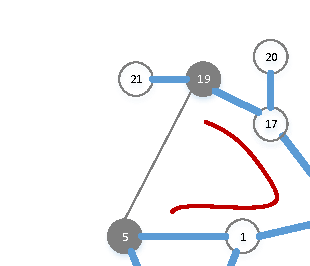
\includegraphics[width=\linewidth]{../figures/new_illustrate/sc_illustrate.pdf}
%    \caption{Edges that do not exist in indexes cannot be explored while estimating shortest paths solely from labels of source and target vertices.}
%    \label{fig:sc_illustrate}
%\end{figure}
%
%In most cases, landmark based algorithms only encode information on a small portion of edges into the indexes. Therefore, edges that have not been encoded into the index are usually the source of estimation errors. As an example, in Fig.\ref{fig:sc_illustrate}, assuming vertex $0$ is the landmark, bold lines represent edges that have been encoded in the index, other lines represent those are not been encoded in the index. Since paths estimated from indexes only contains edges been encoded in the index. Although vertex $4$ and $9$ are adjacent in the underlying graph, the edge connecting them does not exist in the index. So the path estimated solely by the index, which is  will not reflect the true distance of vertex $4$ and $9$. Even edges that are not directly connected with these edges may also be effected, for example from vertex $6$ to $18$, shortest path $(6, 3, 12, 7, 18)$ cannot being extracted directly from the index due to both $(3, 12)$ and $(12, 7)$ are not in indexes. Even though we are dealing with sparse graphs, number of edges been encoded in index for each landmark are less than the number of vertices which are usually much smaller than total number of edges. Thus a lot of edges will be excluded from the index. Simply increasing the number of landmarks will encode more edges in the index, thus will have more accurate results. But clearly, doing so will also bring much more overheads.


We achieve our goal of low-overhead timely query processing with a few design choices. First, instead of estimating shortest path solely from labels of source and target vertices, our algorithm performs a heuristic search during online query period to explore edges that have not been encoded in the index of the network to achieve higher accuracy with limited index size. The heuristic search that we use is called decentralized search which was introduced by \cite{Kleinberg:2000p5066} inspired by the ``greedy heuristic'' that individuals in the small world experiment adopted to find paths to unknown targets. Here the ``decentralized'' means that the decision at each step is made based solely on local information which, in our context, is the labels of neighbor vertices.

Compared to other online searching algorithms, decentralized search is very light-weighted. The number of visited vertices for decentralized search is bounded by two times of diameter of the graph. Considering that complex networks have relatively short diameter, decentralized search can finish the searching in very limited steps. Also, the algorithm does not need to mark which vertices have been visited like BFS or A* search, so very limited space overhead is required for each search. This property makes it possible for large number of searches running in parallel without reaching the memory limit of machines. For example, in our experiments, we showed that nearly millions of decentralized search can run in parallel. One clear drawbacks of decentralized search is that since the speed is traded with relatively small searching space, it can only find approximated shortest paths.

Decentralized search works in a way to explore edges that are not encoded in the index to achieve better accuracy. But its decision for each step is still solely depending on information in the index. So the quality of indexes are still very important for decentralized search to achieve better performance. When constructing indexes, only a small portion of edges can be included. Actually not all the edges are equally important for estimating the shortest path. So which edge should be encoded in the index is a very important problem. By encoding more important edges in the index, without increasing space overhead, the estimation accuracy can be increased.

Our contributions can be summarized as follows:

First, as an approximation algorithm, we combined decentralized search with landmark based indexes to improve the accuracy of landmark based algorithms. We optimized decentralized search based on the structure of index to achieve better accuracy and lower overheads.

Second, we propose a more effective heuristic approach for constructing indexes of the network which can improve the accuracy of the decentralized search without increasing preprocessing overheads.

Third, We construct our algorithm in an distributed manner and perform the decentralized search in a parallel way to further reduce the online query time to achieve better scalability.

The remaining of this paper is organized as follows:
